\section{Montaje}
\begin{figure}[!hb]
	\centering

	\begin{subfigure}[t]{0.4\textwidth}
		\centering
		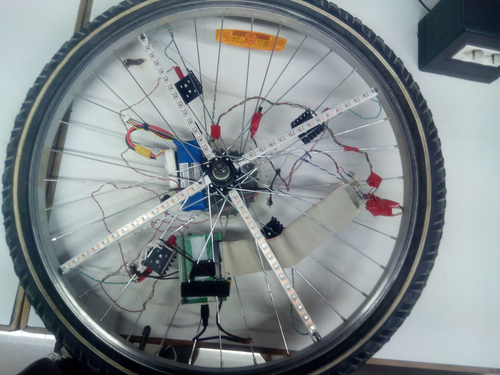
\includegraphics[width=\textwidth]{images/rueda-front}
		\caption{Sistema montado visto de frente}
		\label{fig:rueda-front}
	\end{subfigure}
	\hspace{0.5cm}
	\begin{subfigure}[t]{0.4\textwidth}
		\centering
		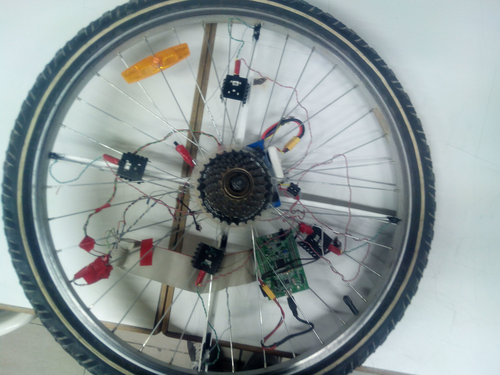
\includegraphics[width=\textwidth]{images/rueda-back}
		\caption{Sistema montado visto desde atrás}
		\label{fig:rueda-back}
	\end{subfigure}

	\caption{Imágenes del sistema montado}
	\label{fig:rueda}
\end{figure}

\subsection{Placa STM32F4-Discovery}
Hemos utilizado la placa STM32F4-Discovery para controlar el sistema. Como
sistema de sujeción se han utilizado tiras adhesivas de Velcro y elásticos, tal
y como se aprecia en la figura \ref{fig:montajePlaca}.

Al principio se comenzó el desarrollo con una PCB de diseño propio con LEDs
paralelos. Más adelante se sustituyó por las tiras de LEDs RGB direccionables.

Para las conexiones se ha utilizando un cable IDE, de esta forma nos aseguramos
un buen contacto con los pines de la paca. El esquemático de este conector se
muestra en la figura \reffig{fig:montajePlaca-IDEsch}.

\begin{figure}[!ht]
	\begin{subfigure}[t]{0.3\textwidth}
		\centering
		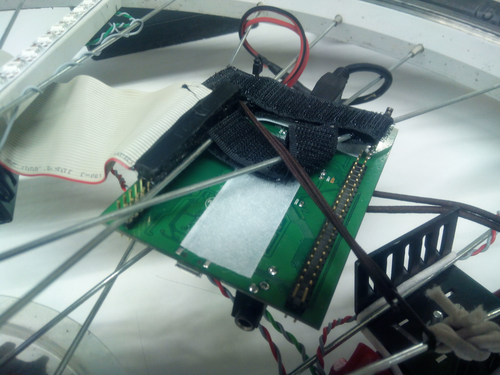
\includegraphics[width=\textwidth]{images/montajePlaca-velcro}
		\caption{Montaje con Velcro y del conector IDE}
		\label{fig:montajePlaca-velcro}
	\end{subfigure}
	\hspace{0.5cm}
	\begin{subfigure}[t]{0.3\textwidth}
		\centering
		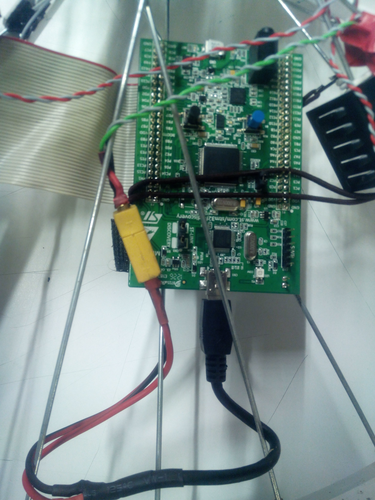
\includegraphics[width=\textwidth]{images/montajePlaca-alimentacion}
		\caption{Conector de alimentación de la placa}
		\label{fig:montajePlaca-alimentacion}
	\end{subfigure}
	\hspace{0.5cm}
	\begin{subfigure}[t]{0.3\textwidth}
		\centering
		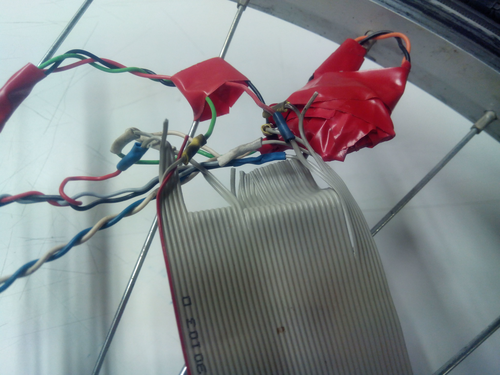
\includegraphics[width=\textwidth]{images/montajePlaca-IDE}
		\caption{Conexión de los periféricos al cable IDE}
		\label{fig:montajePlaca-IDE}
	\end{subfigure}

	\caption{Detalles del montaje de la placa}
	\label{fig:montajePlaca}
\end{figure}

\begin{figure}[!ht]
	\centering
	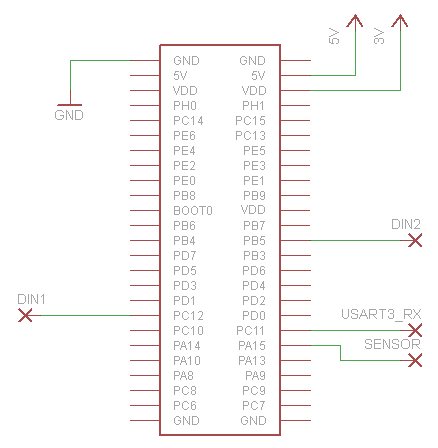
\includegraphics[width=0.6\textwidth]{images/montajePlaca-IDEsch}
	\caption{Esquemático del conector IDE.}
	\label{fig:montajePlaca-IDEsch}
\end{figure}

\newpage
\subsection{LEDs Paralelos}
\label{sec:leds_paralelos}
Antes de utilizar las tiras de LEDs direccionables (ver
\refcont{sec:leds_direccionables}), se utilizó una PCB de diseño propio con 15
LEDs SMD(\reffig{fig:ledsParalelos-front}), un giroscopio y un conector
apropiado (\reffig{fig:ledsParalelos-back}) para los pines de la placa.

También se llegó a crear una aplicación con \uCOS\ que mostraba texto
(\reffig{fig:ledsParalelos-hola}).

\begin{figure}[!ht]
	\centering
	\begin{subfigure}[t]{0.4\textwidth}
		\centering
		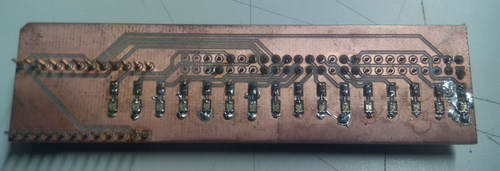
\includegraphics[width=\textwidth]{images/ledsParalelos-front}
		\caption{Detalle de los LEDs SMD}
		\label{fig:ledsParalelos-front}
	\end{subfigure}
	\hspace{0.5cm}
	\begin{subfigure}[t]{0.4\textwidth}
		\centering
		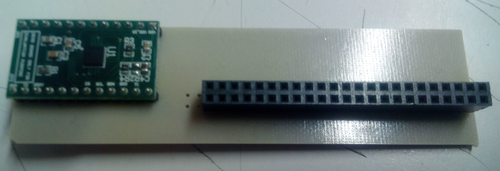
\includegraphics[width=\textwidth]{images/ledsParalelos-back}
		\caption{Detalle del conector y el giroscopio}
		\label{fig:ledsParalelos-back}
	\end{subfigure}
	\\
	\begin{subfigure}[t]{0.3\textwidth}
		\centering
		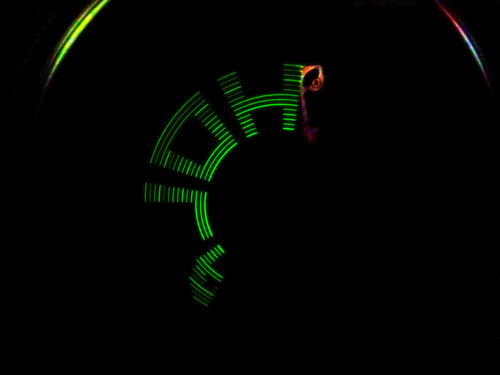
\includegraphics[width=\textwidth]{images/ledsParalelos-hola}
		\caption{Foto de la placa mostrando la palabra ``Hola''}
		\label{fig:ledsParalelos-hola}
	\end{subfigure}

	\caption{Imágenes de la placa de LEDs Paralelos y de su funcionamiento}
	\label{fig:ledsParalelos}
\end{figure}

\newpage
\subsection{Tira de LEDs direccionables}
\label{sec:leds_direccionables}
Las tiras de LEDs direccionables son las responsables de generar el efecto de
POV al girar. Hemos montado 4 tiras de 14 LEDs cada una formando una cruz
perpendicular (\reffig{fig:rueda-front}). Las tiras se encuentran desfasadas dos
a dos, es decir, los LEDs de una tira se encuentran alineados con los de su tira
opuesta, y desfasados con los de su tira perpendicular. De esta forma un LED
pasa justo entre dos de los de su tira desfasada, multiplicando así la
resolución. Igualmente, un LED va a pasar por el mismo sitio que su homologo de
su tira alineada, esto permite reforzar el efecto de POV.

Las tiras se han pegado a unos ``perfiles'' de PVC a los que se le han recortado
muescas para hacerlos encajar entre los radios de la bicicleta
(\reffig{fig:tiraLEDs-sujecion}).

\begin{figure}[!ht]
	\centering

	\begin{subfigure}[t]{0.4\textwidth}
		\centering
		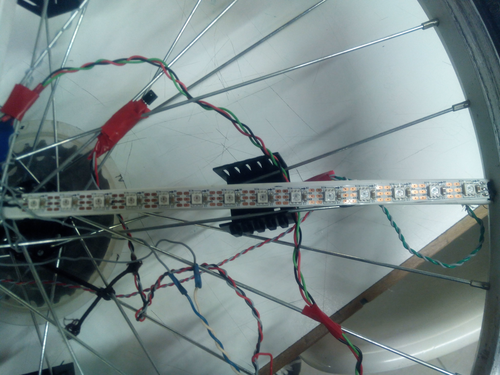
\includegraphics[width=\textwidth]{images/tiraLEDs-completa}
		\caption{Imagen de una tira de LEDs}
		\label{fig:tiraLEDs-completa}
	\end{subfigure}
	\hspace{0.5cm}
	\begin{subfigure}[t]{0.4\textwidth}
		\centering
		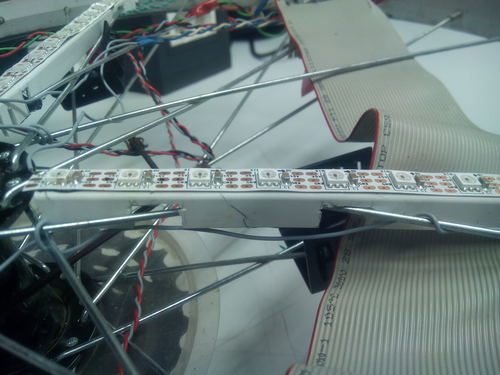
\includegraphics[width=\textwidth]{images/tiraLEDs-sujecion}
		\caption{Detalle de la sujeción de la tira a los radios}
		\label{fig:tiraLEDs-sujecion}
	\end{subfigure}

	\caption{Montaje de una tira de LEDs}
	\label{fig:tiraLEDs}
\end{figure}

Los niveles de voltaje de las tiras son distintos a los de la placa, por lo que
hemos tenido que recurrir a un circuito de conversión de niveles. Éste lo hemos
implementado con buffer. El esquemático se muestra en la figura
\reffig{fig:tiraLEDs-driver}

\begin{figure}[!ht]
	\centering
	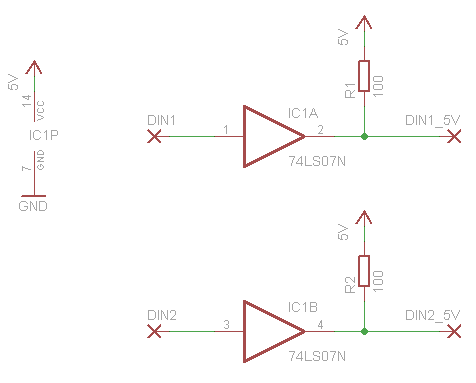
\includegraphics[width=0.7\textwidth]{images/tiraLEDs-driver}
	\caption{Esquemático del driver de conversión de niveles}
	\label{fig:tiraLEDs-driver}
\end{figure}

\newpage
\subsection{Sensores de paso de vuelta}
Para poder dibujar una imagen necesitamos conocer (o estimar) la posición de la
rueda, para así poner en cada LED el color apropiado en el instante apropiado.
Esto lo conseguimos con un sensor de paso de vuelta, a partir del cual
determinamos la velocidad angular a la que gira la rueda, y estimamos la
posición de cada tira durante una vuelta.

Hemos probado dos tipos de sensores de paso de vuelta, un interruptor de
lengüeta (reed switch) (\reffig{fig:pasoVuelta-reedSwitch}) y un sensor de
efecto Hall (\reffig{fig:pasoVuelta-hall}). Debido al los ruidos de rebote
obtenidos con el interruptor de lengüeta, hemos decidido usar el sensor de
efecto Hall.

Al principio pensamos utilizar también un giroscopio para poder reaccionar ante
las variaciones de velocidad durante una vuelta de la rueda, pero dado que este
es un comportamiento poco habitual en una bicicleta y que hemos obtenido muy
buenos resultados con el sensor de paso de vuelta, descartamos esta opción
(\reffig{fig:ledsParalelos-back}).

\begin{figure}[!ht]
	\centering

	\begin{subfigure}[t]{0.4\textwidth}
		\centering
		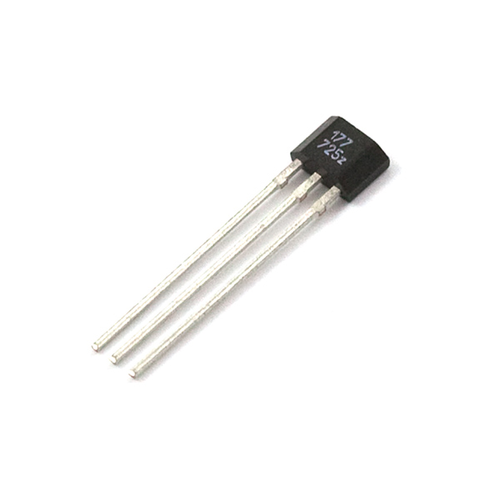
\includegraphics[width=\textwidth]{images/pasoVuelta-hall}
		\caption{Sensor de efecto Hall}
		\label{fig:pasoVuelta-hall}
	\end{subfigure}
	\hspace{0.5cm}
	\begin{subfigure}[t]{0.4\textwidth}
		\centering
		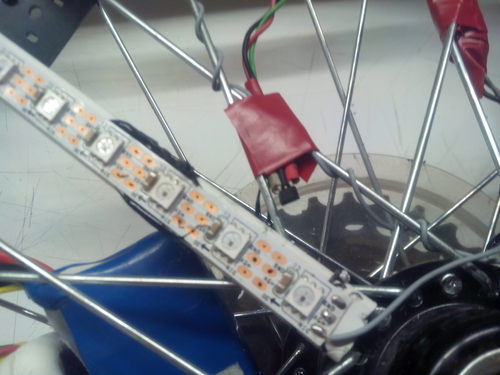
\includegraphics[width=\textwidth]{images/pasoVuelta-montaje}
		\caption{Detalle del montaje en la rueda}
		\label{fig:pasoVuelta-montaje}
	\end{subfigure}
	\\
	\begin{subfigure}[t]{0.5\textwidth}
		\centering
		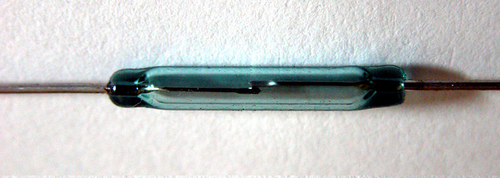
\includegraphics[width=\textwidth]{images/pasoVuelta-reedSwitch}
		\caption{Interruptor de lengüeta. Las dos lengüetas se unen al
		imantarse}
		\label{fig:pasoVuelta-reedSwitch}
	\end{subfigure}

	\caption{Imágenes de los dos tipos de sensores probados y del montaje}
	\label{fig:pasoVuelta}
\end{figure}

\subsection{Receptor y emisor de infrarrojos}
\begin{figure}[!ht]
	\centering

	\begin{subfigure}[t]{0.4\textwidth}
		\centering
		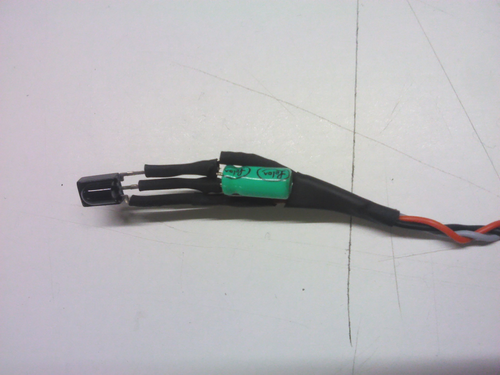
\includegraphics[width=\textwidth]{images/comunicacion-receptor}
		\caption{Receptor IR con condensador de desacople}
		\label{fig:comunicacion-receptor}
	\end{subfigure}
	\hspace{0.5cm}
	\begin{subfigure}[t]{0.4\textwidth}
		\centering
		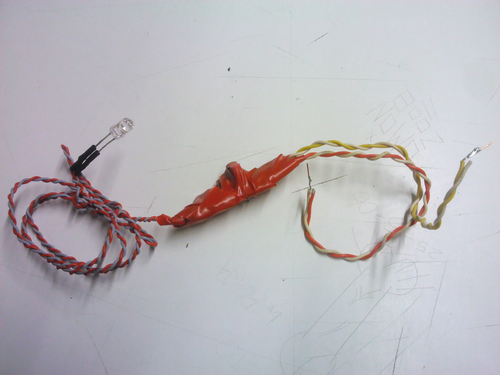
\includegraphics[width=\textwidth]{images/comunicacion-emisor}
		\caption{Emisor conectado al circuito para amplificar y
		modular}
		\label{fig:comunicacion-emisor}
	\end{subfigure}
	\\
	\begin{subfigure}[t]{0.5\textwidth}
		\centering
		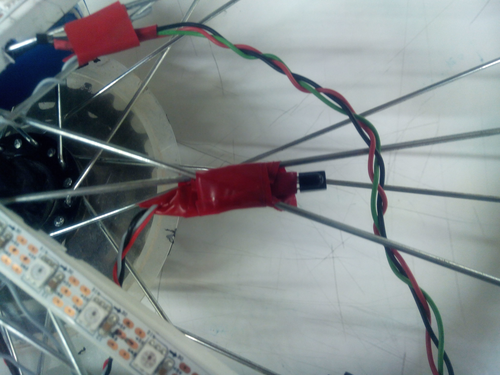
\includegraphics[width=\textwidth]{images/comunicacion-montaje}
		\caption{Detalle del montaje del receptor en la rueda}
		\label{fig:comunicacion-montaje}
	\end{subfigure}

	\caption{Imágenes del los emisores y receptores de infrarrojos}
	\label{fig:comunicacion}
\end{figure}

Para comunicarnos con el sistema mientras está en funcionamiento se hace
necesario un sistema de comunicación inalámbrico. Hemos elegido comunicarnos por
infrarrojos por ser un sistema barato y sencillo de comunicación.

En principio la comunicación será unidireccional desde el PC al sistema en la
bicicleta y solo se transmitirán comandos para cambiar entre imágenes. Más
adelante se pretende implementar la transmisión de imágenes y animaciones junto
con una comunicación half-duplex con ACK.

El receptor de infrarrojos simplemente va conectado a un puerto serie de la
placa, mientras que el emisor necesita un circuito para modular y amplificar la
señal que emite el LED. La señal moduladora a \textsl{38KHz} la generaremos con un
timer de la placa, y la activaremos o desactivaremos directamente con el USART.
Se ha diseñado este circuito para que el LED solo se active cuándo se envíe un
0, ya que el estado en reposo del USART es un 1. El receptor pone su salida a 0
cuando recibe la señal de \textsl{38KHz}, por lo que no necesitamos invertir en ningún
extremo. El esquemático de este circuito se muestra en la figura
\reffig{fig:comunicacion-IRsch}


\begin{figure}[!ht]
	\centering
	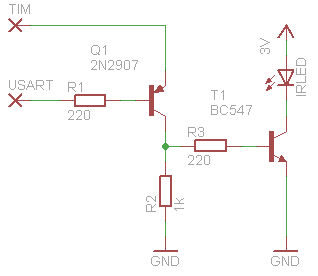
\includegraphics[width=0.7\textwidth]{images/comunicacion-IRsch}
	\caption{Esquemático del circuito modulador y amplificador de
	la señal de infrarrojos.}
	\label{fig:comunicacion-IRsch}
\end{figure}
